\let\lesson\undefined
\newcommand{\lesson}{\phantomlesson{Bài 20: Định luật bảo toàn động lượng.}}
\chapter[Định luật bảo toàn động lượng]{Định luật bảo toàn động lượng}
\setcounter{section}{0}
\section{Lý thuyết}
\subsection{Khái niệm hệ kín (hệ cô lập)}
Một hệ được xem là hệ kín khi hệ đó không có tương tác với các vật bên ngoài hệ.

Ngoài ra, khi tương tác của các vật bên ngoài hệ lên hệ bị triệt tiêu hoặc không đáng kể so với tương tác giữa các thành phần của hệ, hệ vẫn có thể được xem gần đúng là hệ kín.


\subsection{Định luật bảo toàn động lượng}
Động lượng của một hệ kín là một đại lượng bảo toàn.
\begin{equation*}
	\vec{p}_{\text{trước}}=\vec{p}_{\text{sau}}
\end{equation*}

Nếu hệ cô lập gồm hai vật tương tác nhau, công thức trên trở thành:
\begin{equation*}
	\vec{p_1}+\vec{p_2} = \vec{p'_1}+\vec{p'_2},
\end{equation*}
trong đó: 
\begin{itemize}
	\item $	\vec{p_1}$, $\vec{p_2}$ là các vectơ động lượng của hai vật trước khi tương tác;
	\item $	\vec{p'_1}$, $\vec{p'_2}$ là các vectơ động lượng của hai vật sau khi tương tác.
\end{itemize}
\luuy{Nếu một hệ không cô lập nhưng không chịu ngoại lực tác dụng theo một phương, thì ta cũng có thể áp dụng định luật bảo toàn động lượng cho hệ theo phương đó. }
\subsection{Vận dụng định luật bảo toàn động lượng đối với hai vật va chạm mềm}
\begin{center}
	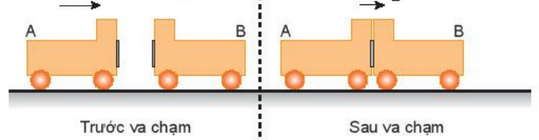
\includegraphics[scale=0.8]{../figs/G10-024-1}
\end{center}

Vật khối lượng $m_1$ chuyển động trên mặt phẳng ngang, nhẵn với vận tốc $\vec{v_1}$, đến va chạm với một vật khối lượng $m_2$ đang có vận tốc $v_2$. 

Sau va chạm, hai vật dính vào nhau, chuyển động với cùng một vận tốc $\vec{v}$.

Va chạm này gọi là va chạm mềm.

Áp dụng định luật bảo toàn động lượng:
\begin{equation*}
	m_1\vec{v}_1+ m_2\vec{v}_2 = (m_1+m_2)\vec{v}.
\end{equation*}
Suy ra 
\begin{equation*}
	\vec{v}=\dfrac{m_1\vec{v}_1+m_2\vec{v}_2}{m_1+m_2}.
\end{equation*}
\luuy{Trong va chạm mềm, cơ năng của hệ không bảo toàn vì một phần cơ năng của hệ đã chuyển hoá thành các dạng năng lượng khác như: năng lượng liên kết các vật với nhau, nhiệt lượng sinh ra ở bề mặt tiếp xúc của các vật khi va chạm, \dots}
\subsection{Vận dụng định luật bảo toàn động lượng đối với hai vật va chạm đàn hồi}

Vật khối lượng $m_1$ chuyển động theo chiều dương trên mặt phẳng ngang, nhẵn với vận tốc $\vec{v_1}$, đến va chạm với một vật khối lượng $m_2$ chuyển động ngược chiều dương với vận tốc $\vec{v_2}$. 

Sau va chạm, các vật tiếp tục chuyển động tách rời nhau với vận tốc $\vec v'_1$ và $\vec v'_2$.

Va chạm được gọi là va chạm tuyệt đối đàn hồi nếu sau va chạm các vật lấy lại hình dạng ban đầu. Trong va chạm tuyệt đối đàn hồi, ngoài bảo toàn động lượng còn có thêm sự bảo toàn cơ năng. 

Để tìm trạng thái các vật sau va chạm, ta phải giải hệ gồm hai phương trình:
\begin{itemize}
	\item Phương trình bảo toàn động lượng 
	\begin{equation*}
		m_1\vec{v_1}+ m_2\vec{v_2} = m_1\vec{v_1'}+m_2\vec{v_2'}.
	\end{equation*}
	\item Phương trình bảo toàn cơ năng 
	\begin{align*}
		\dfrac{1}{2}m_1v_1^2+\dfrac{1}{2}m_2v_2^2=\dfrac{1}{2}m_1(v_1')^2+\dfrac{1}{2}m_2(v_2')^2
	\end{align*}
\end{itemize}
\luuy{
	Trong khi va chạm, lực tương tác giữa các vật va chạm được xem là lớn hơn rất nhiều so với tương tác giữa các vật đó với môi trường bên ngoài, do đó thế năng của các vật được bỏ qua, cơ năng của hệ chỉ gồm động năng các vật thành phần.
}
\subsection{Vận dụng định luật bảo toàn động lượng đối với chuyển động bằng phản lực}
\textbf{Bài toán: }Một tên lửa lúc đầu đứng yên, sau khi lượng khí với khối lượng $m$ phụt ra phía sau với vận tốc $\vec{v}$, thì tên lửa với khối lượng $M$ chuyển động với vận tốc $\vec{V}$.

Áp dụng định luật bảo toàn động lượng 
\begin{equation*}
	\vec{V}= - \dfrac{m}{M} \vec{v}.
\end{equation*}
\luuy{Tên lửa bay lên phía trước ngược với hướng khí phụt ra, không phụ thuộc vào môi trường bên ngoài là không khí hay chân không. Đó là nguyên tắc của chuyển động bằng phản lực.}

\section{Mục tiêu bài học - Ví dụ minh họa}
\begin{dang}{Áp dụng định luật bảo toàn động lượng trong các bài toán va chạm}
	\ppgiai{
		\begin{description}
			\item[Bước 1] Xác định hệ cô lập, viết phương trình bảo toàn động lượng cho hệ cô lập (hệ kín):
			\begin{equation*}
				\vec{p_1}+\vec{p_2}+\vec{p_3}+ \ldots =\vec{p'_1}+\vec{p'_2}+\vec{p'_3}+ \ldots ;
			\end{equation*}
			\item [Bước 2] Thiết lập các phương trình hình chiếu trên các trục tọa độ O$x$ và O$y$:
			\begin{equation*}
				\begin{cases}
					p_{1x}+p_{2x}+p_{3x}+ \ldots &= p'_{1x}+p'_{2x}+p'_{3x}+ \ldots;\\
					p_{1y}+p_{2y}+p_{3y}+ \ldots &= p'_{1y}+p'_{2y}+p'_{3y}+ \ldots;
				\end{cases}
			\end{equation*}
			
			\item [Bước 3] Giải các phương trình hình chiếu, thu được giá trị đại lượng cần tìm.
			Trong một số trường hợp (va chạm đàn hồi) cần phải kết hợp thêm định luật bảo toàn cơ năng. 
		\end{description}
	}
	\viduii{2}{Một vật khối lượng $m$ đang chuyển động theo phương ngang với vận tốc $v$ thì va chạm vào vật khối lượng $2m$ đang đứng yên. Sau va chạm, hai vật dính vào nhau và chuyển động với cùng vận tốc. Bỏ qua ma sát, vận tốc của hệ hai vật sau va chạm là
		\begin{mcq}(4)
			\item $\dfrac{v}{3}$. 
			\item $v$.
			\item $3v$.
			\item $\dfrac{v}{2}$.
		\end{mcq}
	}
	{	\begin{center}
			\textbf{Hướng dẫn giải}
		\end{center}
		Áp dụng định luật bảo toàn động lượng cho hệ vật $m$, $2m$ ngay trước và sau va chạm:
		$$m\vec v+ \vec 0=\left(m+2m\right)\vec V$$
		$$\Rightarrow \vec V=\dfrac{\vec v}{3}$$
		Như vậy, sau va chạm hệ vật chuyển động cùng chiều chuyển động ban đầu của vật $m$ với tốc độ $V=\dfrac{v}{3}$.
		
		\textbf{Đán án: A}.
		
		\begin{center}
			\textbf{Câu hỏi tương tự}
		\end{center}
		
		Một vật khối lượng $m_1=\SI{1}{kg}$ chuyển động thẳng đều trên mặt phẳng nằm ngang với tốc độ $\SI{12}{m/s}$ và va chạm với vật có khối lượng $m_2=\SI{2}{kg}$ đang đứng yên. Sau va chạm, hai vật dính chặt với nhau. Bỏ qua mọi ma sát. Tốc độ của hai vật sau va chạm là
		\begin{mcq}(4)
			\item $\SI{4}{m/s}$. 
			\item $\SI{6}{m/s}$.
			\item $\SI{12}{m/s}$.
			\item $\SI{24}{m/s}$.
		\end{mcq}
		
		\textbf{Đáp án: A}.
	}
	\viduii{3}{Vật $m_1$ chuyển động với tốc độ $\SI{6}{\meter/\second}$ đến va chạm với vật $m_2$ chuyển động ngược chiều với tốc độ $\SI{2}{\meter/\second}$. Sau va chạm, hai vật bật ngược trở lại với cùng tốc độ $\SI{4}{\meter/\second}$. Tính khối lượng của hai vật biết $m_1+m_2=\SI{ 1,5}{\kilogram}$.
	}
	{	\begin{center}
			\textbf{Hướng dẫn giải}
		\end{center}
		
		Áp dụng định luật bảo toàn động lượng cho hệ vật $m_1$, $m_2$ ngay trước và sau va chạm
		\begin{equation}
			\label{eq:30.1}
			m_1\overrightarrow{v_1} + m_2\overrightarrow{v_2} = m_1\overrightarrow{v_1'} + m_2\overrightarrow{ v_2'}
		\end{equation}
	Chiếu phương trình (\ref{eq:30.1}) lên chiều chuyển động ban đầu của $m_1$, ta thu được:
	\begin{equation}
		\label{eq:30.2}
		m_1v_1-m_2v_2=-m_1v'_1+m_2v'_2
	\end{equation}
		Từ phương trình (\ref{eq:30.2}) kết hợp với điều kiện $m_1+m_2=\SI{1.5}{\kilogram}$, ta giải được $m_1=\SI{0.5625}{\kilogram}$ và $m_2=\SI{0,9375}{\kilogram}$.
		
		
		\begin{center}
			\textbf{Câu hỏi tương tự}
		\end{center}
		
		Vật $\SI{200}{\gram}$ chuyển động với tốc độ $\SI{6}{\meter/\second}$ đến va chạm với vật $\SI{50}{\gram}$ chuyển động với tốc độ $\SI{4}{\meter/\second}$. Sau va chạm vật $\SI{200}{\gram}$ giữ nguyên hướng chuyển động với tốc độ bằng nửa tốc độ ban đầu. Tính tốc độ của vật còn lại sau va chạm, biết rằng trước va chạm hai vật chuyển động ngược chiều.
		
		\textbf{Đáp án:} $v_2'=\SI{8}{m/s}$.
		
		
	}
\end{dang}

\begin{dang}{Áp dụng định luật bảo toàn động lượng \\trong bài toán chuyển động bằng phản lực}
	\viduii{2}{Một khẩu súng nằm ngang khối lượng $m_\text{s}=\SI{1000}{\kilogram}$, bắn một viên đạn khối lượng $m_\text{đ}=\SI{10}{\gram}$. Vận tốc viên đạn ra khỏi nòng súng là $\SI{600}{\meter/\second}$. Độ lớn vận tốc của súng sau khi bắn bằng là bao nhiêu?
	}
	{	\begin{center}
			\textbf{Hướng dẫn giải}
		\end{center}
		Chọn chiều dương là chiều chuyển động của đạn. 
		
		Áp dụng định luật bảo toàn động lượng cho hệ đạn và súng ngay trước và sau khi bắn:
		\begin{eqnarray*}
			\vec{0}&=&m_\text{đ}\vec v_\text{đ}+m_\text{s}\vec v_\text{s}\\
			\Rightarrow \vec v_\text{s}&=&-\dfrac{m_\text{đ}}{m_\text{s}}\cdot\vec v_\text{đ}
		\end{eqnarray*}
		Dấu trừ cho thấy súng bị giật ngược hướng chuyển động của đạn.\\
		Tốc độ giật lùi của súng:
		$$v_s=\dfrac{m_\text{đ}}{m_\text{s}}\cdot v_\text{đ}=\dfrac{\SI{10E-3}{\kilogram}}{\SI{1000}{\kilogram}}\cdot\left(\SI{600}{\meter/\second}\right)=\SI{6E-3}{\meter/\second}=\SI{0.6}{\centi\meter/\second}.$$
		
		
		\begin{center}
			\textbf{Câu hỏi tương tự}
		\end{center}
		
		Một khẩu súng nằm ngang khối lượng $m_\text{s} = 5\ \text{kg}$, bắn một viên đạn khối lượng $m_\text{đ} = 10\ \text{g}$. Vận tốc viên đạn ra khỏi nòng súng là 600 m/s. Độ lớn vận tốc của súng sau khi bắn bằng
		\begin{mcq}(4)
			\item 12 m/s.	
			\item 6 m/s.
			\item 1,2 m/s.	
			\item 60 m/s.
		\end{mcq}
		
		\textbf{Đáp án: C}.
	}
	\viduii{4}{
		Tên lửa có khối lượng vỏ là 10 tấn chuyển động với vận tốc $\SI{200}{\meter/\second}$ so với Trái Đất, 2 tấn khí phụt ra có vận tốc $\SI{500}{\meter/\second}$ so với tên lửa. Xác định vận tốc của tên lửa sau khi khí phụt ra.
	}
	{\begin{center}
			\textbf{Hướng dẫn giải}
		\end{center}
	Gọi:
	\begin{itemize}
		\item (1) khí phụt ra sau tên lửa;
		\item (2) tên lửa;
		\item (0) mặt đất.
	\end{itemize}
Ta có: $v_{20}=\SI{200}{\meter/\second}$; $v'_{12}=\SI{500}{\meter/\second}$.
		
		Áp dụng định luật bảo toàn động lượng cho hệ tên lửa và khí ngay trước và sau khi khí phụt ra:
	\begin{eqnarray*}
		\left(m_1+m_2\right)\overrightarrow{v_{20}}&=&m_1\overrightarrow{v'_{10}}+m_2\overrightarrow{v'_{20}}\\
		\Leftrightarrow \left(m_1+m_2\right)\overrightarrow{v_{20}}&=&m_1\left(\overrightarrow{v'_{12}}+\overrightarrow{v_{20}}\right)+m_2\overrightarrow{v'_{20}}\\
		\Rightarrow m_2\overrightarrow{v_{20}}&=&m_1\overrightarrow{v'_{12}}+m_2\overrightarrow{v'_{20}} \quad (*)
	\end{eqnarray*}
	Chiếu phương trình (*) lên chiều chuyển động ban đầu của tên lửa, thu được:
	$$m_2v_{20}=-m_1v'_{12}+m_2v'_{20}$$
	$$\Rightarrow v'_{20}=\dfrac{m_2v_{20}+m_1v'_{12}}{m_2}=\dfrac{\left(\SI{10E3}{\kilogram}\right)\cdot\left(\SI{200}{\meter/\second}\right)+\left(\SI{2E3}{\kilogram}\right)\cdot\left(\SI{500}{\meter/\second}\right)}{\SI{10E3}{\kilogram}}=\SI{300}{\meter/\second}.$$
		\begin{center}
			\textbf{Câu hỏi tương tự}
		\end{center}
		
		Tên lửa có khối lượng tổng cộng là 10 tấn chuyển động với vận tốc $\SI{200}{\meter/\second}$ so với Trái Đất, 2 tấn khí phụt ra có vận tốc $\SI{500}{\meter/\second}$ so với tên lửa. Xác định vận tốc của tên lửa sau khi khí phụt ra.
		
		\textbf{Đáp án:} $v_1  =\SI{325}{m/s}$.
	}
\end{dang}
\begin{dang}{Áp dụng định luật bảo toàn động lượng trong các bài toán đạn nổ}
	\viduii{2}{
		Một viên đạn khối lượng $\SI{0.5}{kg}$ đang bay theo phương ngang với vận tốc 1000 m/s thì nổ thành hai mảnh có khối lượng bằng nhau và cùng độ lớn vận tốc bay theo phương vuông góc với nhau. Xác định độ lớn động lượng của mỗi mảnh sau khi nổ.
	}
	{\begin{center}
			\textbf{Hướng dẫn giải}
		\end{center}
		
		\begin{itemize}
			\item Xét hệ gồm hai mảnh đạn trong thời gian nổ, đây được xem là hệ kín nên ta áp dụng định luật bảo toàn động lượng.
			\item Động lượng trước khi đạn nổ
			\begin{equation*}
			\vec{p_{\text{t}}}=m\vec{v}
			\end{equation*}
			\item Động lượng sau khi đạn nổ
			\begin{equation*}
				\vec{p_{\text{s}}}=m_1\vec{v_1}+m_2 \vec{v_2} =\vec{p_1} + \vec{p_2}. 
			\end{equation*}
			\item Vì hai mảnh sau khi nổ có động lượng bằng nhau và vuông góc với nhau nên
			\begin{equation*}
				p^2= p_1^2 + p_2^2 = 2p_1^2 \Rightarrow p = p_1 \sqrt{2} \Rightarrow p_1=p_2=\dfrac{p}{\sqrt{2}}=\SI{353.55}{kg \cdot m/s}.
			\end{equation*}
			
		\end{itemize}
		
		\begin{center}
			\textbf{Câu hỏi tương tự}
		\end{center}
		
		Một viên đạn khối lượng $\SI{1}{kg}$ đang bay theo phương ngang với vận tốc $100\sqrt 2$ m/s thì nổ thành hai mảnh có khối lượng bằng nhau và cùng độ lớn vận tốc, bay theo phương vuông góc với nhau. Xác định độ lớn động lượng của mỗi mảnh sau khi nổ.
		
		\textbf{Đáp án:} $\SI{100}{kg \cdot m/s}$.
	}
	\viduii{3}{Một viên đạn khối lượng 1 kg đang bay theo phương thẳng đứng với tốc độ 500 m/s thì nổ thành hai mảnh có khối lượng bằng nhau. Mảnh thứ nhất bay theo phương ngang với tốc độ 1000 m/s. Động lượng mảnh thứ hai có
		\begin{mcq}
			\item độ lớn $707\ \text{kg} \cdot \text{m/s}$; hướng lên trên tạo với phương ngang một góc $\beta= 60^\circ$.
			\item độ lớn $500\ \text{kg} \cdot \text{m/s}$; hướng lên trên tạo với phương ngang một góc $\beta= 60^\circ$. 
			\item độ lớn $500\ \text{kg} \cdot \text{m/s}$; hướng lên trên tạo với phương ngang một góc $\beta= 45^\circ$. 
			\item độ lớn $707\ \text{kg} \cdot \text{m/s}$; hướng lên trên tạo với phương ngang một góc $\beta= 45^\circ$.
		\end{mcq}
	}
	{	\begin{center}
			\textbf{Hướng dẫn giải}
		\end{center}
		
		\begin{center}
			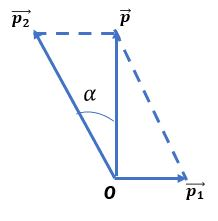
\includegraphics[scale=0.6]{../figs/VN10-PH-29-L-021-4-1.JPG}
		\end{center}
		Xét hệ gồm hai mảnh đạn trong thời gian nổ, đây được xem là hệ kín nên ta áp dụng định luật bảo toàn động lượng.
		
		Động lượng trước khi đạn nổ
		\begin{equation*}
			\vec{p_{\text{t}}} =m\vec{v}=\vec p
		\end{equation*}
		
		Động lượng sau khi đạn nổ
		\begin{equation*}
			\vec{p_{\text{s}}}=m_1\vec{v_1}+m_2 \vec{v_2} =\vec{p_1} + \vec{p_2}. 
		\end{equation*}
		
		Áp dụng định luật bảo toàn động lượng các mảnh vỡ ngay trước và sau khi đạn nổ
		\begin{align*}
			\vec{p}=\vec{p}_1+\vec{p}_2
		\end{align*}
Sử dụng định lý Pythagoras
		
		
		\begin{equation*}
			p^2_2 =p^2+p^2_1 \Rightarrow p_2 \approx\SI{707}{kg \cdot m/s}.
		\end{equation*}
		Góc giữa $\vec v_2$ và phương thẳng đứng: 
		\begin{equation*}
			\sin \alpha = \dfrac{p_1}{p_2} = \dfrac{1}{\sqrt 2} \Rightarrow \alpha = 45^\circ \Rightarrow \beta = 45^\circ.
		\end{equation*}
		
		\textbf{Đáp án: D.}
		
		\begin{center}
			\textbf{Câu hỏi tương tự}
		\end{center}
		
		Một viên đạn khối lượng $\SI{0.5}{kg}$ đang bay theo phương ngang với tốc độ 1000 m/s thì nổ thành hai mảnh có khối lượng bằng nhau. Mảnh thứ nhất bay theo phương thẳng đứng lên trên với tốc độ 1200 m/s. Động lượng mảnh thứ hai có
		\begin{mcq}
			\item độ lớn $464\ \text{kg} \cdot \text{m/s}$; hướng lên trên tạo với phương ngang một góc $\beta= 25^\circ$.
			\item độ lớn $464\ \text{kg} \cdot \text{m/s}$; hướng xuống dưới tạo với phương ngang một góc $\beta= 25^\circ$. 
			\item độ lớn $583\ \text{kg} \cdot \text{m/s}$; hướng lên trên tạo với phương ngang một góc $\beta= 31^\circ$. 
			\item độ lớn $583\ \text{kg} \cdot \text{m/s}$; hướng xuống dưới tạo với phương ngang một góc $\beta= 31^\circ$.
		\end{mcq}
		
		\textbf{Đáp án: D}.
	}
	
\end{dang}